% Chapter 2 text
\chapter{Assessing the blank carbon contribution, isotope mass balance, and kinetic isotope fractionation of the ramped pyrolysis/oxidation instrument at NOSAMS}
\label{Ch2}
\raggedbottom

{\let\thefootnote\relax\footnotetext{This chapter was originally published as: Hemingway J.D., Galy V.V., Gagnon A.R., Grant K.E., Rosengard S.Z., Soulet G., Zigah P.K., and McNichol A.P. (2017) {Assessing the blank carbon contribution, isotope mass balance, and kinetic isotope fractionation of the ramped pyrolysis/oxidation instrument at NOSAMS.} \emph{Radiocarbon} \textbf{under review.} }}

\clearpage

\section{Abstract}

We estimate the blank carbon mass over the course of a typical Ramped PyrOx (RPO) run ($150 - 1000$\textdegree C; $5$\textdegree C min\textsuperscript{-1}) to be $3.7 \pm 0.6$ $\mu$gC with an Fm value of $0.555 \pm 0.042$ and a $\delta^{13}$C value of $-29.0 \pm 0.1$\textperthousand\ VPDB. Additionally, we provide equations for RPO Fm and $\delta^{13}$C blank corrections, including associated error propagation. By comparing RPO mass-weighted mean and independently measured bulk \ce{\delta^{13}C} values for a compilation of environmental samples and standard reference materials (SRMs), we observe a small yet consistent \ce{^{13}C} depletion within the RPO instrument (mean -- bulk: $\mu = -0.8$\textperthousand; $\pm 1 \sigma$ = $0.9$\textperthousand; $n = 66$). In contrast, mass-weighted mean Fm values accurately match bulk measurements (mean -- bulk: $\mu = 0.005$; $\pm 1 \sigma$ = $0.014$; $n = 36$). Lastly, we show there exists no significant intra-sample \ce{\delta^{13}C} variability across carbonate SRM peaks, indicating minimal mass-dependent kinetic isotope fractionation during RPO analysis. These data are best explained by a difference in activation energy between \ce{^{12}C}- and \ce{^{13}C}-containing compounds ($\Delta E$) of $0.3 - 1.8$ J mol\textsuperscript{-1}, suggesting that blank and mass-balance corrected RPO \ce{\delta^{13}C} values accurately retain carbon source isotope signals to within $1 - 2$\textperthousand.

\section{Introduction}

Thermoanalytical instruments such as thermogravimetry (TG) and pyrolysis gas chromatography (pyGC) are frequently used in petroleum geoscience \citep{Peters:1986uc}, biofuels research \citep{White:2011iz}, and soil science \citep{Plante:2009cp} to monitor the thermal reactivity of organic carbon (OC) contained within environmental samples. Additionally, petroleum geochemists have long coupled thermal analysis methods with isotope ratio measurements to investigate the origins and maturity of thermogenic hydrocarbons, leading to the development of techniques such as pyGC-isotope ratio mass spectrometry \citep[IRMS;][]{Galimov:1988vq,Berner:1996wn,Cramer:2004tg}. However, despite their potential to probe the relationship between OC molecular composition, isotope composition, and thermal reactivity, coupled thermal-isotope methods have found limited use in other fields of organic geochemistry. Still, preliminary studies analyzing environmental samples such as soils indicate that TG coupled with IRMS can yield meaningful trends in stable-carbon ($^{13}$C) composition with temperature \citep{LopezCapel:2006bc,LopezCapel:2008et}. Furthermore, \citet{Szidat:2004kx} and \citet{Currie:2005wo} successfully separated and determined the radiocarbon (\ce{^{14}C}) content of organic and elemental ("black") carbon fractions in aerosols using a stepped-temperature approach, confirming the possibility that thermal-isotope techniques can be used in tandem with radiocarbon analysis.

Recently, a novel instrument has been developed at NOSAMS to determine both the stable and radiocarbon isotope composition of evolved gases from environmental samples with increasing temperature \citep{Rosenheim:2008ed}. This method, termed "Ramped PyrOx" or "RPO", is increasingly being utilized in a host of environments to understand the relationship between carbon source, \ce{^{14}C} content, and thermal reactivity \citep[\textit{e.g.}][]{Rosenheim:2012kh,Plante:2013tu,Rosenheim:2013dka,Schreiner:2014jr,Bianchi:2015jr}. However, a complete understanding of isotope fractionation within the RPO instrument is currently lacking, hindering our ability to accurately interpret evolved-gas \ce{^{13}C} composition as a carbon source tracer. Additionally, RPO analysis shows promise for improving age-model constraints on carbonate-free sediments \citep{Rosenheim:2013va,Subt:2016dh}, although this application requires that contaminant ("blank") carbon contributions and \ce{^{14}C} mass balance are well constrained. Therefore, the aim of this study is to investigate the blank carbon contribution, isotope mass balance, and kinetic fractionation within the RPO instrument located at NOSAMS.

\section{Analytical Setup}

The NOSAMS RPO instrumental design is originally described in \citet{Rosenheim:2008ed} and has since been modified to lower contaminant carbon inputs by replacing all plumbing with copper tubing, improve gas flow rates, and improve temperature ramp stability \citep{Plante:2013tu}. In this setup, ultra-high purity (UHP) He gas flows at $32$ mL min\textsuperscript{-1} into a pre-combusted ($850$\textdegree C, 5 hours) quartz reactor sitting in a two-stage oven containing sample material to be pyrolyzed/oxidized (Figure \ref{Ch2Fig:1}A--B). He gas is combined with $3$ mL min\textsuperscript{-1} UHP O\textsubscript{2} either $(i)$ prior to entering the quartz reactor ("oxidation mode") or $(ii)$ downstream of sample material but upstream of a Cu, Pt, and Ni wire catalyst via a reactor side-arm ("pyrolysis mode"). An optimized, combined flow rate of $35$ mL min\textsuperscript{-1} was chosen to minimize transfer time within the system while still allowing sufficient contact time with the wire catalyst and complete cryogenic trapping of CO\textsubscript{2}. During a run, the lower oven containing the catalyst is held at $800$\textdegree C to facilitate oxidation of reduced carbon-containing gases to \ce{CO2}, while the upper oven containing the sample is ramped at a user-defined rate with $\approx 5$\% precision (typically $5 \pm 0.2$\textdegree C min\textsuperscript{-1}). We note that care must be taken when analyzing HCl-fumigated soil/sediment samples \citep[\textit{e.g.}][]{Plante:2013tu} as well as marine sediments and dissolved OC, as residual chloride has been observed to interact with and melt the catalysis wire, thus blocking gas flow within the reactor.

After exiting the ovens, water vapor is removed using a dry ice and isopropanol slurry. Gases are then passed into an in-line Sable Systems\textsuperscript{\textregistered} CA-10 infrared gas analyzer (IRGA) where \ce{CO2} concentration (in parts per million by volume, ppm\ce{CO2}) is measured photometrically at 1-second resolution with $\approx 5$ ppm\ce{CO2} precision in order to generate a plot of temperature vs. \ce{CO2} concentration (termed a "thermogram"). Finally, gases are transferred to a toggling trap apparatus (Figure \ref{Ch2Fig:1}A, \ref{Ch2Fig:1}C--D) in which \ce{CO2} is frozen using liquid \ce{N2} while \ce{He} and \ce{O2} are vented to the atmosphere. At user-defined temperatures, the collecting trap is toggled and \ce{CO2} for each temperature window (termed a "fraction") is transferred to a vacuum line, quantified manometrically, and sealed into a pre-combusted ($525$\textdegree C, 1 hour) $6$ mm Pyrex\textsuperscript{\textregistered} tube containing $100$ mg \ce{CuO} and $10$ mg \ce{Ag} pellets. Following a run, tubes are re-combusted ($525$\textdegree C, 1 hour) to remove sulfur-containing contaminant gases and \ce{CO2} carbon isotopes are measured following standard NOSAMS procedures \citep{McNichol:1992tk,McNichol:1994dt,Pearson:1998vy}. Between each run, \ce{CO2} concentration measurements are calibrated using a 2-point calibration curve by plumbing $(i)$ UHP \ce{He} and $(ii)$ UHP \ce{He} containing a known \ce{CO2} concentration directly through the IRGA.

% Figure 1
\begin{figure}[t]
	\makebox[\textwidth][c]{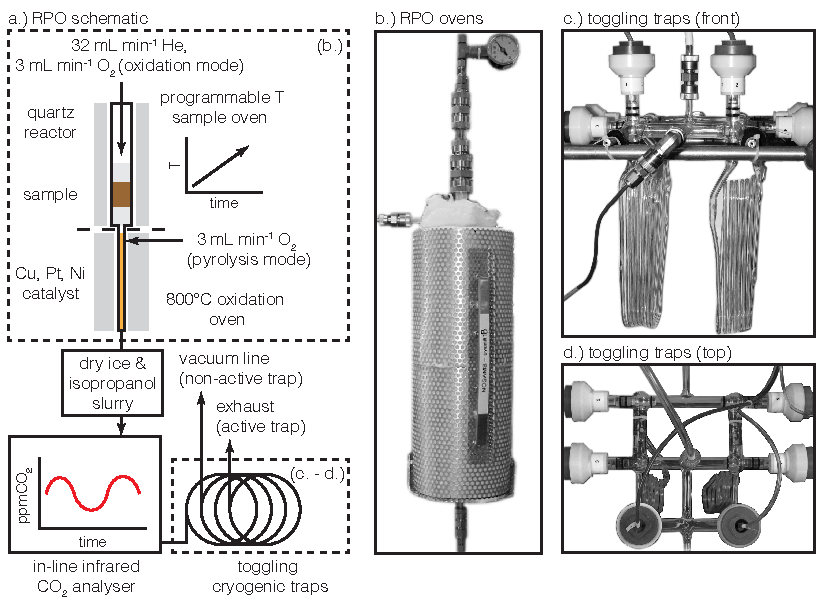
\includegraphics[]{Thesis_Figures/Ch2Fig1}}
	\caption[RPO instrumental setup and photos]{The NOSAMS RPO instrumental setup: $(A)$ schematic diagram, $(B)$ photo of the ovens, and $(C) - (D)$ photos of the toggling trap apparatus. Dashed boxes in panel $(A)$ indicate the regions shown in panels $(B) - (D)$.}
	\label{Ch2Fig:1} 
\end{figure}

\section{Results and Discussion}

\subsection{NOSAMS RPO blank correction}

In order to estimate the RPO blank carbon mass and isotope composition, we directly trapped and analyzed \ce{CO2} eluted from empty, pre-combusted reactor inserts over the temperature range of a typical run ($150 - 1000$\textdegree C). Although blank carbon contribution is often determined by monitoring deflections from accepted standard reference material (SRM) isotope compositions \citep[\textit{i.e.} isotope dilution and "modern-dead" methods;][]{Pearson:1998vy,dosSantos:2007ca,Fernandez:2014gx,ShahWalter:2015iu}, the direct measurement method employed here is better-suited for the RPO instrument for the following reasons: 

\begin{enumerate}[label=(\textit{\roman*})]

\item Deflections from accepted SRM isotope values are only informative over the narrow temperature range in which the material decomposes, rather than over the course of an entire run.

\item For stable isotopes, it is possible that kinetic fractionation could overprint isotope deflections due to blank carbon contribution \citep[\textit{e.g.}][]{Cramer:2004tg,Dieckmann:2005dw}.

\item Isotope deflection methods are unable to separate blank carbon contributed within the quartz reactor \citep[\textit{i.e.} time-dependent blank carbon;][]{Fernandez:2014gx} from that contributed when switching the toggling trap apparatus \citep[\textit{i.e.} time-independent blank carbon;][]{Fernandez:2014gx}.

\end{enumerate}

To address point $(iii)$, we calculated the blank carbon mass and Fm value when the traps were toggled 0, 2, and 5 times between $150$ and $1000$\textdegree C. For 2- and 5-toggle runs, fractions were recombined within the vacuum line before transferring to a $6$ mm Pyrex tube to keep subsequent steps identical across all experimental conditions. Each experiment was performed in duplicate and the \ce{CO2} mass from each run was quantified separately before pairs were combined for ultra-small \ce{^{14}C} analysis \citep{ShahWalter:2015iu}. The 0-toggle experiment was repeated in duplicate for \ce{^{13}C} analysis using a dual-inlet IRMS as described in \citet{McNichol:1994dt}.

Resulting blank carbon mass is independent of the number of toggles throughout the run (Table \ref{Ch2Tab:1}), averaging $3.7 \pm 0.6$ $\mu$gC ($n = 8$) and indicating that the act of toggling the traps contributes a negligible amount of time-independent blank carbon. This is further supported by the near-identical Fm values across experimental conditions (Table \ref{Ch2Tab:1}). We therefore combine measurements from all experiments and calculate an average blank carbon Fm value of $0.555 \pm 0.042$ ($n = 3$). Similarly, we assume that the measured 0-toggle blank carbon \ce{\delta^{13}C} value of $-29.0 \pm 0.1$\textperthousand\ relative to Vienna Pee Dee Belemnite (VPDB; Table \ref{Ch2Tab:1}) is applicable regardless of the number of toggles.

% Table 1
\begin{sidewaystable}[p]
	\caption[RPO blank carbon mass, flux, and isotope composition]{NOSAMS RPO blank carbon mass, flux, and isotope composition. For measurements with $n = 1$, reported std. dev. is instrumental uncertainty. For measurements with $n = 2$, reported std. dev. is $\frac{1}{2}$ of the range between values.}
	\centering
		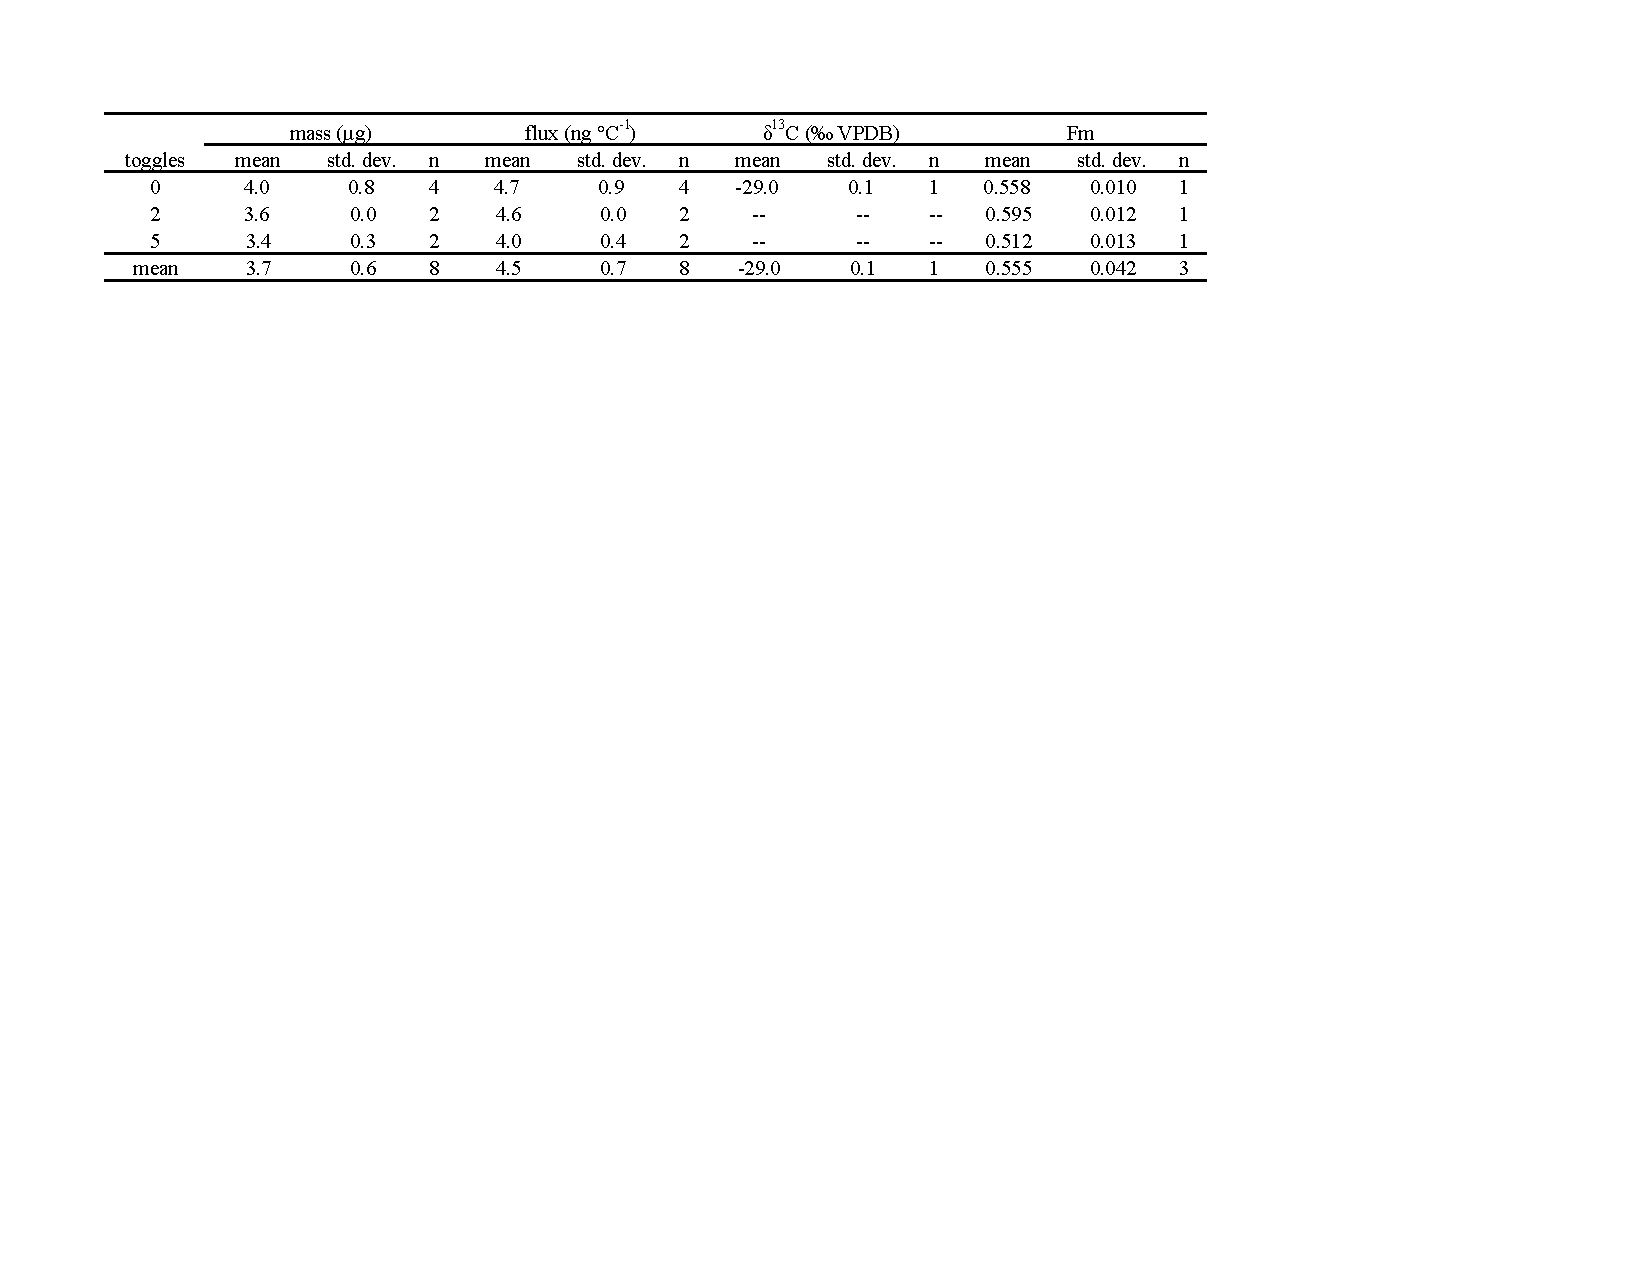
\includegraphics{Thesis_Tables/Ch2Tab1}
	\label{Ch2Tab:1}
\end{sidewaystable}

Blank carbon mass calculated here is significantly lower and less variable than that determined for a similar RPO system \citep[\textit{c.f.} $12.9 \pm 7.0$ $\mu$gC;][]{Fernandez:2014gx}, likely due to recent valve and plumbing upgrades on the NOSAMS instrument \citep{Plante:2013tu}. Additionally, photometric measurements suggest that time-dependent blank carbon contribution is not concentrated within any particular temperature range -- that is, there exist no distinct peaks in the blank thermograms (Figure \ref{Ch2Fig:2}). Although the mean blank flux appears to drop slightly above $500$\textdegree C, it can nonetheless be reasonably described as constant throughout the run within the 95\% confidence interval of the manometric measurements (Figure \ref{Ch2Fig:2}). Dividing the blank carbon mass by the experimental temperature range results in a blank carbon flux of $4.5 \pm 0.7$ ngC \textdegree C\textsuperscript{-1} (assuming a $5$\textdegree C min\textsuperscript{-1} ramp rate; Table \ref{Ch2Tab:1}). We therefore correct the mass of carbon in each RPO fraction for blank contribution according to:

% Equation 1
\begin{equation}\label{Ch2Eq:1}
m_{s} = m_{m} - \phi_{b} \Delta T
\end{equation}

where $m_{s}$ is the true sample carbon mass, $m_{m}$ is the measured carbon mass, $\phi_{b}$ is the blank carbon flux (in units of mass \textdegree C\textsuperscript{-1}), and $\Delta T$ is the temperature range over which the \ce{CO2} was collected. Additionally, we propagate uncertainty for this correction according to:

% Equation 2
\begin{equation}\label{Ch2Eq:2}
\sigma_{m_{s}} = \sqrt{ \left( \sigma_{m_{m}} \right)^2 + \left( \sigma_{\phi_{b}} \Delta T \right)^2}
\end{equation}
 
where $\sigma$ is the standard deviation associated with each subscripted measurement. This assumes that $\Delta T$ is known perfectly (\textit{i.e.} $\Delta T \equiv 0.0$) and that the uncertainty in $m_{m}$ and $\phi_{b}$ are uncorrelated, which is reasonable given that $m_{s} \approx m_{m} >> \Delta T \phi_{b}$. Similarly, we treat the measured \ce{CO2} isotope composition as a weighted average of sample carbon and blank carbon, and correct for blank contribution following:

% Equation 3
\begin{equation}\label{Ch2Eq:3}
\ce{^{x}R}_{s} = \frac{m_{m} \ce{^{x}R}_{m} - \phi_{b} \Delta T \ce{^{x}R}_{b}}{m_{s}}
\end{equation}

where $\ce{^{x}R}_{i}$ is the $\ce{^{x}C}/\ce{^{12}C}$ isotope ratio of component $i$ [$x$ = 13, 14; $i$ = (s)ample, (m)easured, (b)lank], with $\ce{^{13}R}_{i}$ expressed in \ce{\delta^{13}C} notation (\textperthousand\ VPDB) and $\ce{^{14}R}_{i}$ expressed in Fm notation \citep{Stuiver:1977uh,Reimer:2004th}. Lastly, we propagate uncertainty associated with isotope corrections. Because $m_{s} \approx m_{m}$, we cancel these where appropriate to avoid large covariance terms, leading to the equation:

% Equation 4
\begin{equation}\label{Ch2Eq:4}
\sigma_{\ce{^{x}R}_{s}} \approx \sqrt{\left( \sigma_{\ce{^{x}R}_{m}} \right)^2 + \left( \frac{\Delta T \ce{^{x}R}_{b}}{m_{s}} \sigma_{\phi_{b}} \right)^2 + \left( \frac{\phi_{b} \Delta T}{m_{s}} \sigma_{\ce{^{x}R}_{b}} \right)^2 + \left( \frac{\phi_{b} \Delta T \ce{^{x}R}_{b}}{m_{s}^{2}} \sigma_{m_{s}} \right)^2}
\end{equation}

For typical RPO fraction \ce{CO2} masses ($\approx 100$ $\mu$gC) and $\Delta T$ ($\approx 100$\textdegree C) encountered during sample runs, blank carbon correction shifts \ce{\delta^{13}C} values by $-0.02$ (for $\ce{\delta^{13}C} = -35$\textperthousand\ VPDB) to $+0.15$\textperthousand\ (for $\ce{\delta^{13}C} = +5$\textperthousand\ VPDB) and Fm values by $-0.002$ (for Fm = $0.01$) to $+0.002$ (for Fm = $1.0$), within the typical analytical uncertainty of these measurements. While \ce{^{14}C} content of graphite targets containing as little as $6$ $\mu$gC has been accurately analyzed at NOSAMS \citep{ShahWalter:2015iu}, we recommend a minimum RPO fraction mass of $25$ $\mu$gC in order to keep blank carbon corrections below $0.5$\textperthousand\ for \ce{\delta^{13}C} and $0.01$ for Fm (assuming $\Delta T = 100$\textdegree C). %A spreadsheet for performing all blank correction calculations is included in the supplementary material (Table S1).

% Figure 2
\begin{figure}[t]
	\makebox[\textwidth][c]{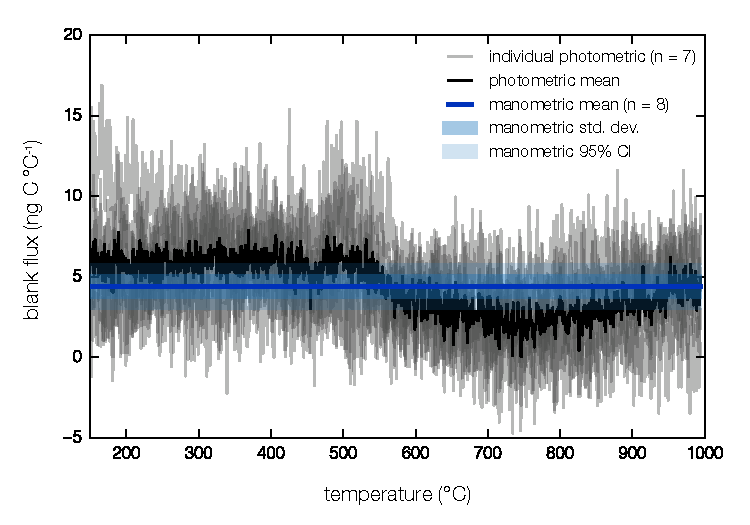
\includegraphics[]{Thesis_Figures/Ch2Fig2}}
	\caption[RPO blank carbon flux]{RPO blank carbon flux for a ramp rate of $5$\textdegree C min\textsuperscript{-1} as determined photometrically and manometrically. For photometric measurements, absolute \ce{CO2} concentrations were normalized such that the mean value for each run is equal to the manometric mean, as small differences in IRGA baseline calibration between runs leads to large changes in calculated blank flux. Still, photometric measurements are consistent with a constant flux throughout the run.}
	\label{Ch2Fig:2} 
\end{figure}

\subsection{Isotope mass balance}

If sample carbon is completely converted to \ce{CO2} by the end of a run and is efficiently transferred to the vacuum line, the mass-weighted mean \ce{CO2} isotope composition of blank-corrected RPO fractions should match independently measured bulk values within analytical uncertainty. To test this, we compare RPO mass-weighted mean compositions with bulk measurements for a range of sample types (SRMs, dissolved organic carbon, fluvial/marine total suspended sediments, soils, and lacustrine/marine sediments). Bulk \ce{\delta^{13}C} values were obtained either using an elemental analyzer coupled to a continuous-flow IRMS following \citet{Whiteside:2011jea} or on a dual-inlet IRMS after conversion to \ce{CO2} by closed-tube combustion as described in \citet{McNichol:1994dt}. Bulk Fm was measured at NOSAMS following standard preparation methods for each sample type \citep{McNichol:1994ty} and uncertainty for each bulk measurement is taken as the measured analytical uncertainty. We calculate RPO mass-weighted mean isotope compositions ($\mean{\ce{^{x}R}_{s}}$) as:

% Equation 5
\begin{equation}\label{Ch2Eq:5}
\mean{\ce{^{x}R}_{s}} = \Sigma_{j=1}^{n} f_{j} \ce{^{x}R}_{s,j}
\end{equation}

where $n$ is the total number of \ce{CO2} fractions collected throughout the run, $f_{j}$ is the contribution of fraction $j$ to the total mass of \ce{CO2} such that $\Sigma_{j=1}^{n} f_{j} \equiv 1.0$, and $\ce{^{x}R}_{s,j}$ is the blank-corrected $\ce{^{x}C}/\ce{^{12}C}$ isotope ratio of fraction $j$. Additionally, assuming that $f_{j}$ is known perfectly (\textit{i.e.} since $\Sigma_{j=1}^{n} f_{j}$ must equal $1.0$ by definition), we estimate the mass-weighted mean isotope uncertainty according to:

% Equation 6
\begin{equation}\label{Ch2Eq:6}
\sigma_{\mean{\ce{^{x}R}_{s}}} \approx \sqrt{ \Sigma_{j=1}^{n} \left( f_{j} \sigma_{\ce{^{x}R}_{s,j}} \right)^2}
\end{equation}

To test the ability of RPO mass-weighted mean isotope values to predict measured bulk values, we performed orthogonal distance regression (ODR), including uncertainty in both $x$ and $y$ variables, using the SciPy package in Python v3.5. and a weighting factor for each sample that is inversely proportional to the uncertainty in each measurement \citep{Boggs:1990wc,Oliphant:2007ud}. All data presented here are either taken from the literature \citep{Rosenheim:2012kh,Rosenheim:2013va} or are originally presented in this study.

% Figure 3
\begin{figure}[t]
	\makebox[\textwidth][c]{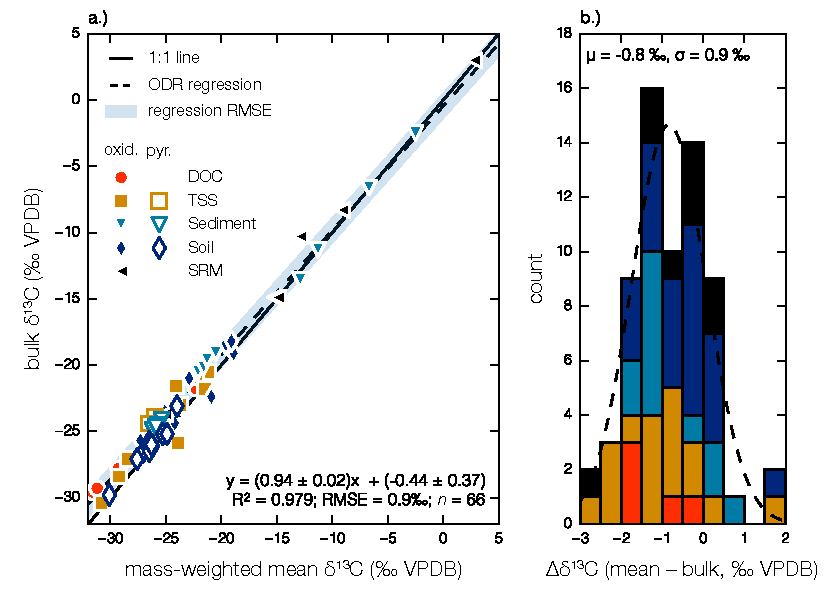
\includegraphics[]{Thesis_Figures/Ch2Fig3}}
	\caption[RPO \ce{\delta^{13}C} mass balance]{$(A)$ cross-plot of RPO mass-weighted mean vs. independently measured bulk \ce{\delta^{13}C} values for all samples in this study in which \ce{\delta^{13}C} data exist and $(B)$ the same data presented as a histogram of deviations from bulk values ($\Delta \ce{\delta^{13}C} = \ce{\delta^{13}C}_{\text{mean}} - \ce{\delta^{13}C}_{\text{bulk}}$). Sample abbreviations are as follows: DOC, dissolved organic carbon; TSS, total suspended sediments; SRM, standard reference material.}
	\label{Ch2Fig:3} 
\end{figure}

\subsubsection{Stable isotope mass balance}

On average, the RPO mass-weighted mean composition is depleted in \ce{^{13}C} by $0.8 \pm 0.9$\textperthousand\ relative to bulk measurements ($n = 66$), independent of RPO run conditions (Figure \ref{Ch2Fig:3}), as has been described previously \citep{Rosenheim:2012kh,Rosenheim:2013va}. To test if residual \ce{^{13}C}-enriched carbon remaining after RPO analysis could cause this depletion, \citet{Rosenheim:2012kh} re-quantified the carbon content of total suspended sediment samples after ramping to $1000$\textdegree C and determined that only $\approx 0.003$\% of initial carbon remained. Therefore, for the samples tested therein, \citet{Rosenheim:2012kh} concluded that low yield could not explain the observed bias. We tested additional potential sources of this depletion by performing a series of experiments using a \ce{CO2}:\ce{He} calibration gas mixture with known isotope composition ($465.5$ ppm\ce{CO2} in \ce{He}, $\ce{\delta^{13}C} = -14.9 \pm 0.04$\textperthousand\ VPDB) by:

\begin{enumerate}[label=(\textit{\roman*})]

\item Plumbing calibration gas directly into the toggling traps (bypassing the ovens of the RPO system) over a range of flow rates: $15$, $35$, and $50$ mL min\textsuperscript{-1}.

\item Freezing \ce{CO2} from the calibration gas for a range of integration times for each of the flow rates in experiment $(i)$: 1, 5, and 10 minutes.

\item Plumbing calibration gas through an empty, pre-combusted reactor insert and collecting \ce{CO2} between $150$ and $1000$\textdegree C, toggling every $170$\textdegree C for a total of 5 fractions (flow rate = $35$ mL min\textsuperscript{-1}, ramp rate = $5$\textdegree C min\textsuperscript{-1}).

\end{enumerate}

The results of experiments $(i)$ and $(ii)$ reveal that, for all flow rates and integration times, the collected \ce{CO2} \ce{\delta^{13}C} value ($-15.0 \pm 0.1$\textperthousand, $n = 9$) is statistically identical to the accepted value, indicating that dynamic cryogenic trapping within the toggling traps imparts no isotope fractionation. Furthermore, oven temperature does not appear to affect \ce{^{13}C} composition, as \ce{\delta^{13}C} values from all fractions in experiment $(iii)$ are statistically identical with a mean value of $-15.2 \pm 0.04$\textperthousand\ ($n = 5$). Although this is $0.3$\textperthousand\ depleted relative to the accepted value, this bias is smaller than that observed in most samples within our sample set (\textit{i.e.} up to $3$\textperthousand, Figure \ref{Ch2Fig:3}B), suggesting that any fractionation imparted during transport through the hot oven alone cannot cause observed \ce{^{13}C} depletion.

However, we note that the mass-weighted mean vs. bulk \ce{\delta^{13}C} difference is more pronounced in decarbonated samples containing exclusively OC (mean -- bulk: $\mu = -1.0$\textperthousand; $\pm 1\sigma =  0.9$\textperthousand; $n = 60$) as compared either to samples containing mixtures of carbonate and OC or pure carbonate SRMs (mean -- bulk: $\mu = -0.1$\textperthousand; $\pm 1\sigma =  0.5$\textperthousand; $n = 6$). We therefore hypothesize that isotope fractionation during OC degradation within the RPO oven could cause \ce{^{13}C} depletion, potentially due to incomplete oxidation to \ce{CO2} while reduced carbon-containing gases are in contact with the catalyst wire (Figure \ref{Ch2Fig:1}A). This mechanism is consistent with the results of experiment $(iii)$ indicating a lack of temperature dependence on isotope fractionation. We therefore recommend that \ce{\delta^{13}C} values of each RPO fraction $j$ within a particular sample can be fractionation-corrected according to the difference between mass-weighted mean and bulk measurements of that sample:

% Equation 7
\begin{equation}\label{Ch2Eq:7}
\ce{\delta^{13}C}_{s,j,\text{corrected}} = \ce{\delta^{13}C}_{s,j} + \left( \ce{\delta^{13}C}_{\text{bulk}} - \mean{\ce{\delta^{13}C}_{s}} \right)
\end{equation}

Furthermore, assuming that the covariance between $\ce{\delta^{13}C}_{s,j}$ for each fraction $j$ and the mass-weighted mean value ($\mean{\ce{\delta^{13}C}_{s}}$) is small compared to all other variance terms, we propagate uncertainty associated with fractionation correction according to:

% Equation 8
\begin{equation}\label{Ch2Eq:8}
\sigma_{\ce{\delta^{13}C}_{s, j, \text{corrected}}} \approx \sqrt{\sigma_{\ce{\delta^{13}C}_{s,j}}^2 + \sigma_{\ce{\delta^{13}C}_{\text{bulk}}}^2 + \sigma_{\mean{\ce{\delta^{13}C}_{s}}}^2 }
\end{equation}

\subsubsection{\ce{^{14}C} mass balance}

% Figure 4
\begin{figure}[t]
	\makebox[\textwidth][c]{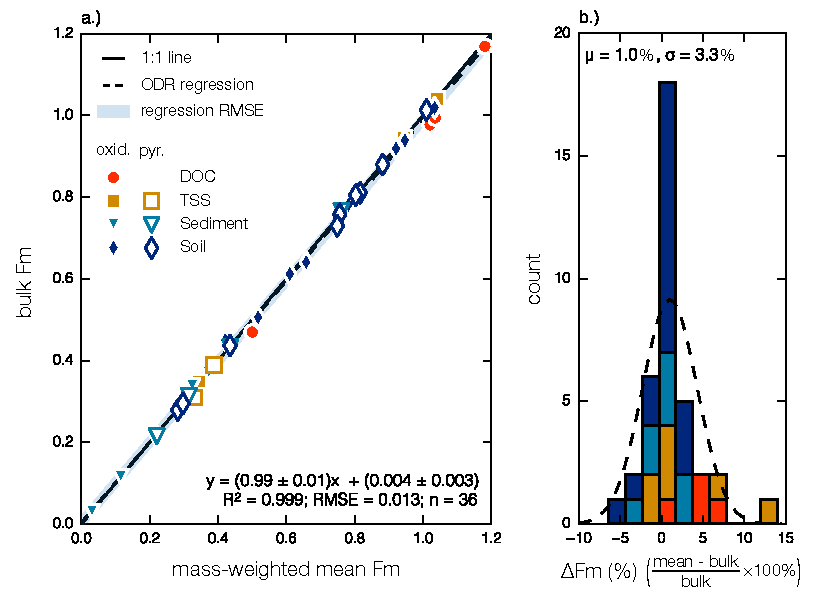
\includegraphics[]{Thesis_Figures/Ch2Fig4}}
	\caption[RPO Fm mass balance]{$(A)$ cross-plot of RPO mass-weighted mean vs. independently measured bulk Fm values for all samples in this study in which Fm data exist and $(B)$ the same data presented as a histogram of relative deviations from bulk values, in percent ($\Delta$Fm (\%) = $\frac{\text{Fm}_{\text{mean}} - \text{Fm}_{\text{bulk}}}{\text{Fm}_{\text{bulk}}} \times 100$\%). Sample abbreviations are as follows: DOC, dissolved organic carbon; TSS, total suspended sediments.}
	\label{Ch2Fig:4} 
\end{figure}

In contrast to \ce{^{13}C}, mass-weighted mean Fm values typically agree with bulk Fm values within analytical uncertainty across all sample types and run conditions (mean -- bulk: $\mu = 0.005$; $\pm 1 \sigma = 0.014$; $n = 36$; Figure \ref{Ch2Fig:4}). This can be easily explained because Fm is by definition corrected for the \ce{^{13}C}/\ce{^{12}C} ratio as measured on the AMS \citep{Stuiver:1977uh,dosSantos:2007ca} such that any mass-dependent fractionation occurring in the RPO instrument is accounted for. It is additionally useful to compare relative deviations between bulk and RPO mean values, as \ce{^{14}C} content of samples is highly variable. For the samples analyzed here, this equates to an average mean -- bulk relative difference of 1.0\% with a standard deviation of 3.3\% ($n = 36$), independent of absolute \ce{^{14}C} content of the sample (Figure \ref{Ch2Fig:4}B). This agreement between the mass-weighted mean Fm and bulk Fm values further precludes the possibility that a significant amount of isotopically unique carbon remains unreacted after ramping to $1000$\textdegree C, and is strong evidence that \ce{^{14}C} mass balance during RPO analysis is robust over the entire range of Fm values found in nature.

\subsection{Kinetic fractionation}

Finally, we evaluate the kinetic isotope effect (KIE) due to mass-dependent differences in pyrolysis/oxidation rates between each isotope during temperature ramping. If the amplitude of the KIE is significant relative to natural compositional differences, changes in \ce{\delta^{13}C} values between RPO fractions within a single sample can reflect instrumental fractionation rather than differences in carbon source isotope composition. Quantifying fractionation due to the KIE is therefore critical in order to interpret \ce{^{13}C} composition as a carbon source tracer. To do so, we measured \ce{\delta^{13}C} values of eluted \ce{CO2} from two carbonate SRMs in high-resolution fashion by toggling every $\approx 20$\textdegree C: $(i)$ travertine calcite \citep[IAEA C2;][]{Rozanski:1992vp} and $(ii)$ Icelandic spar (in-house standard; long-term average $\ce{\delta^{13}C} = 3.00 \pm 0.03$\textperthousand). Because carbonates are chemically and isotopically homogenous, any resulting \ce{\delta^{13}C} variability should follow a predictable, Rayleigh-like fractionation line that depends only on the difference in activation energy ($E$) between the decomposition of \ce{^{12}C}- and \ce{^{13}C}-containing molecules \citep[$\Delta E = \ce{^{13}E} - \ce{^{12}E}$;][]{Kwart:1982te}. We describe the carbonate decomposition rate constant at any temperature [k($T$)] by an Arrhenius equation (here written for \ce{^{12}C}):

% Equation 9
\begin{equation}\label{Ch2Eq:9}
\ce{^{12}k}(T) = \ce{^{12}A} \exp \left( - \frac{\ce{^{12}E}}{RT} \right)
\end{equation}

where \ce{^{12}A} is the Arrhenius pre-exponential factor for \ce{^{12}C} and $R$ is the ideal gas constant. Following \citet{Kwart:1982te}, the KIE at any temperature [KIE($T$)] is defined as the ratio of \ce{^{12}C} and \ce{^{13}C} rate constants at that temperature: 

% Equation 10
\begin{equation}\label{Ch2Eq:10}
\text{KIE}(T) = \frac{\ce{^{12}k}(T)}{\ce{^{13}k}(T)} = \left( \frac{\ce{^{12}A}}{\ce{^{13}A}} \right) \exp \left( \frac{\Delta E}{RT} \right)
\end{equation}

Equation \ref{Ch2Eq:10} fundamentally states that, for a given $\Delta E$, \ce{^{12}A}, and \ce{^{13}A}, KIE($T$) decreases with increasing $T$, indicating that kinetic fractionation within the RPO instrument will be largest for lower temperature components. Furthermore, we can reasonably assume that entropic differences between \ce{^{12}C}- and \ce{^{13}C}-containing molecules are negligible within the carbonate crystal lattice \citep[\textit{c.f.}][]{Tang:2000ua}. This assumption implies that $\ce{^{12}k}(T) = \ce{^{13}k}(T)$ as $T$ approaches infinity and requires that $\ce{^{12}A} = \ce{^{13}A} = A$ \citep{Cramer:2004tg}. Additionally, for each temperature we compute the \ce{^{13}C} composition of the remaining carbonate that has not yet decomposed [$\ce{^{13}R_{carb}}(T)$] as:

% Equation 11
\begin{equation}\label{Ch2Eq:11}
\ce{^{13}R_{carb}}(T) = \mean{\ce{^{13}R}_{s}} \exp \left( \frac{\ce{^{12}I}(T) - \ce{^{13}I}(T)}{\beta} \right)
\end{equation}

where $\beta$ is the oven ramp rate, $\mean{\ce{^{13}R}_{s}}$ is the mass-weighted mean \ce{^{13}C} content of the sample calculated by Equation \ref{Ch2Eq:5}, and $\ce{^{12}I}(T)$ and $\ce{^{13}I}(T)$ are the temperature integrals for \ce{^{12}C}- and \ce{^{13}C}-containing molecules according to \citet{Braun:1987vf} (here written for \ce{^{12}C}):

% Equation 12
\begin{equation}\label{Ch2Eq:12}
\ce{^{12}I}(T) \approx \frac{RT^2}{\ce{^{12}E}} \ce{^{12}k}(T) = \frac{ART^2}{\ce{^{12}E}} \exp \left( - \frac{\ce{^{12}E}}{RT} \right)
\end{equation}

Finally, following \citet{Cramer:2004tg}, we calculate the predicted \ce{^{13}C} composition of instantaneously eluted \ce{CO2} at any temperature [$\ce{^{13}R_{CO_2}}(T)$]:

% Equation 13
\begin{equation}\label{Ch2Eq:13}
\ce{^{13}R_{CO_2}}(T) = \frac{\ce{^{13}R_{carb}}(T)}{\text{KIE}(T)} = \ce{^{13}R_{carb}}(T) \exp \left( - \frac{\Delta E}{RT} \right)
\end{equation}

Calculating $\ce{^{13}R_{CO_2}}(T)$ requires two inputs in addition to $\Delta E$: $A$ and \ce{^{12}E}. Here we prescribe $A$ \textit{a priori} and estimate \ce{^{12}E} for each SRM by minimizing the root mean squared error (RMSE) between predicted first-order decay rates and observed thermograms using a Nelder-Mead algorithm in the SciPy package for Python v3.5. \citep[Table \ref{Ch2Tab:2};][]{Nelder:1965tk,Oliphant:2007ud}. We note that $\ce{^{13}R_{CO_2}}(T)$ is insensitive to our choice of $A$ \citep{Dieckmann:2005dw,White:2011iz}. For example, assuming a large $\Delta E$ value of $100$ J mol\textsuperscript{-1} for a peak at $700$\textdegree C, changing $A$ from $10^{10}$ sec\textsuperscript{-1} to $10^{20}$ sec\textsuperscript{-1} increases \ce{\delta^{13}C} of the first 1\% of eluted \ce{CO2} by only $1$\textperthousand\ and the first 50\% of eluted \ce{CO2} by only $0.2$\textperthousand. We therefore reasonably choose $A = 10^{15}$ sec\textsuperscript{-1} based on a compilation of literature values \citep[see][for review]{White:2011iz}. We then calculate $\Delta E$ that best predicts the \ce{^{13}C} composition of all \ce{CO2} fractions for each SRM by minimizing the measured vs. predicted RMSE \citep{Nelder:1965tk,Oliphant:2007ud}. To accurately compare instantaneous \ce{^{13}C} content predicted by Equation \ref{Ch2Eq:13} to measured RPO fractions (which integrate over time), we use the \ce{CO2}-mass-weighted average temperature for each fraction.

% Table 2
\begin{sidewaystable}[p]
	\caption[$\Delta E$ comparison between RPO and other instruments]{Comparison of $A$, \ce{^{12}E}, and $\Delta E$ values for carbonate SRMs in this study with those calculated using various thermoanalytical techniques on petroleum products \citep{Tang:2000ua,Cramer:2004tg,Tian:2007df}.}
	\centering
		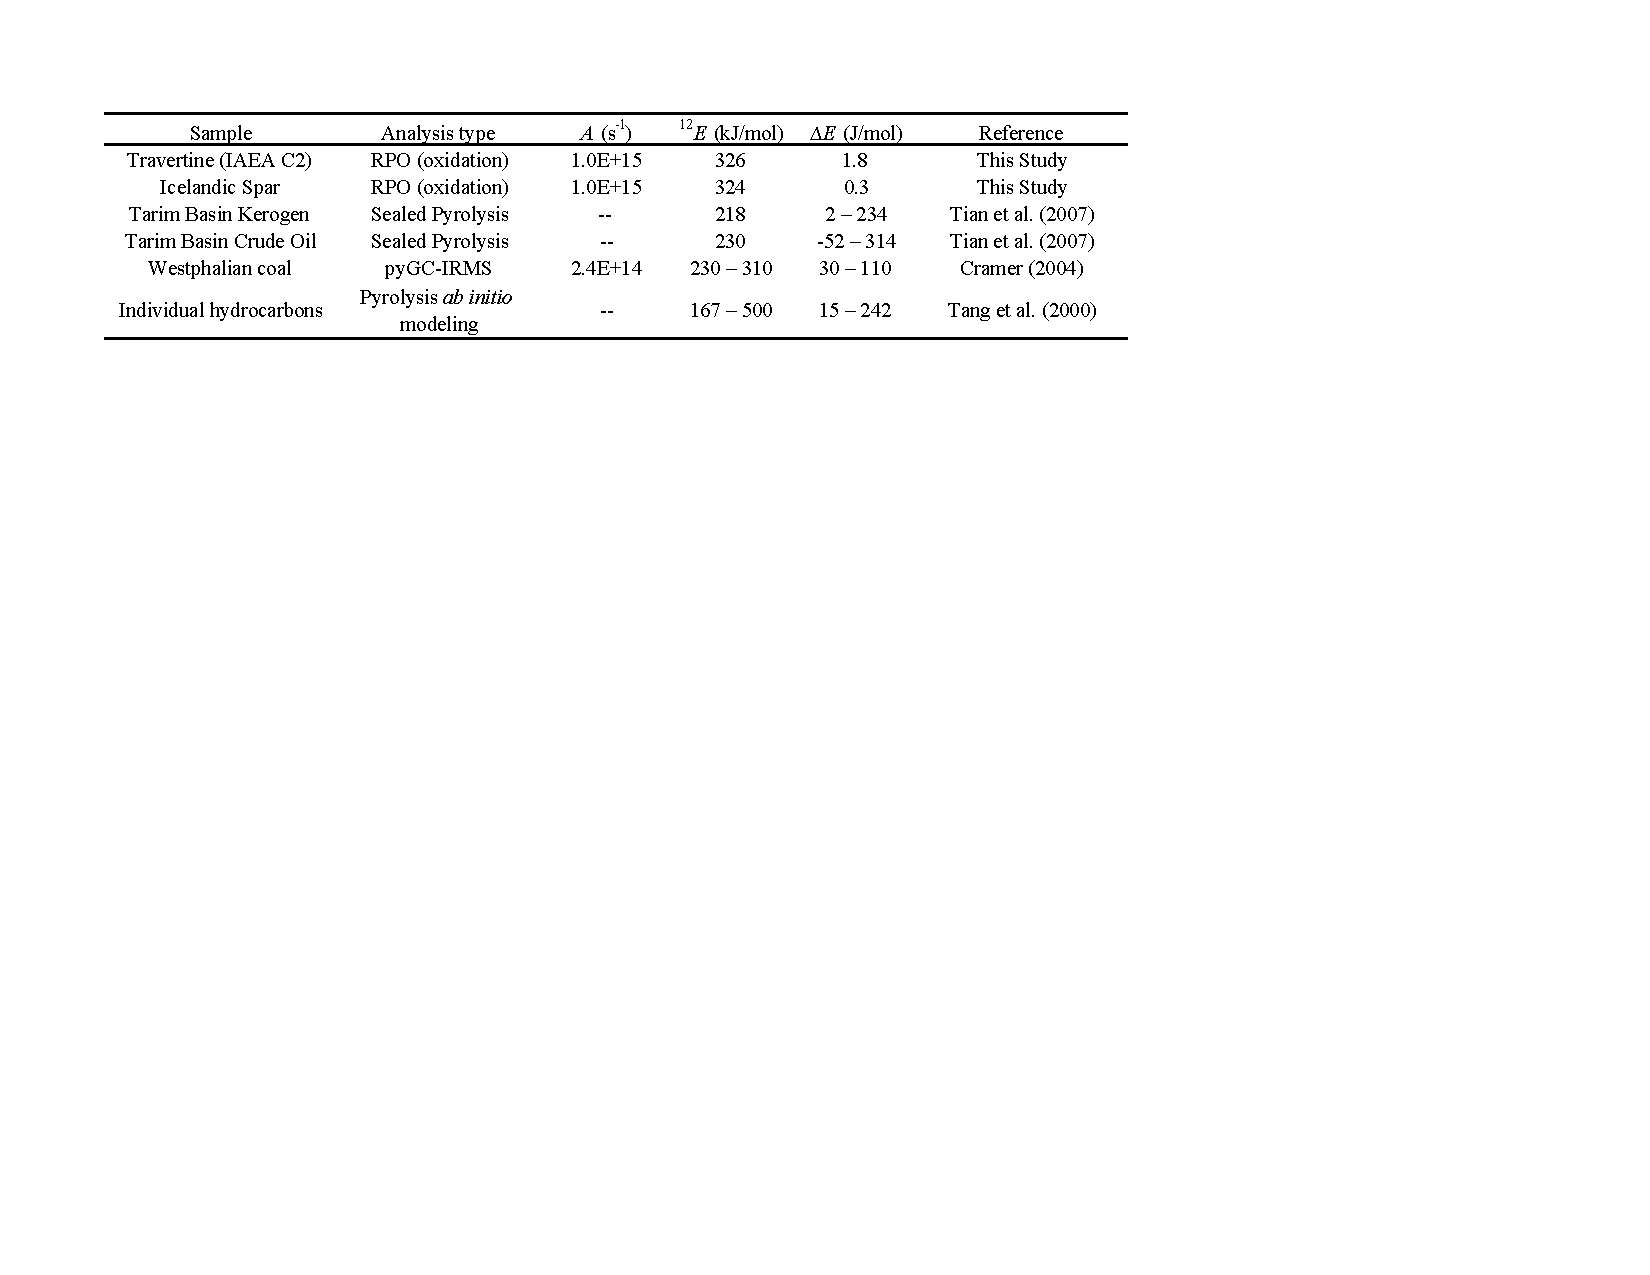
\includegraphics{Thesis_Tables/Ch2Tab2}
	\label{Ch2Tab:2} 
\end{sidewaystable}

Measured \ce{^{13}C} composition for both SRMs is consistent with a $\Delta E$ value between $0.3$ and $1.8$ J mol\textsuperscript{-1} (Table \ref{Ch2Tab:2}; Figure \ref{Ch2Fig:5}), significantly smaller than literature values for petroleum products using various non-isothermal pyrolysis instruments (Table \ref{Ch2Tab:2}). Therefore, for the SRMs analyzed here, predicted \ce{CO2} \ce{\delta^{13}C} increases by $<1$\textperthousand\ until $>>99$\% of initial carbon has been decomposed (Figure \ref{Ch2Fig:5}). However, we note that, on one hand, calculated $\Delta E$ using carbonate SRMs is likely a minimum estimate for environmental samples, as this carbon is already present in a +IV oxidation state, while oxidation of OC could increase $\Delta E$. On the other hand, it has been shown that samples with high molecular diversity -- as is expected in environmental OC mixtures -- exhibit less apparent kinetic isotope fractionation than do single compounds such as the carbonates analyzed here \citep{Cramer:2004tg}. Overall, we recommend that a $\Delta E$ range of $0.3 - 1.8$ J mol\textsuperscript{-1} is valid for any component within an RPO run, and we consequently predict that kinetic isotope fractionation cannot exceed $1.8$\textperthousand\ during pyrolysis/oxidation of the first $99$\% of any sample eluting between $150$ and $1000$\textdegree C. In reality, \ce{^{13}C} enrichment at $>>99$\% combustion will never be observed during RPO analysis, as each fraction typically contains $10 - 20$\% of total carbon. We therefore conclude that \ce{\delta^{13}C} variability greater than $1 - 2$\textperthousand\ between RPO fractions must reflect differences in source carbon isotope composition.

% Figure 5
\begin{figure}[t]
	\makebox[\textwidth][c]{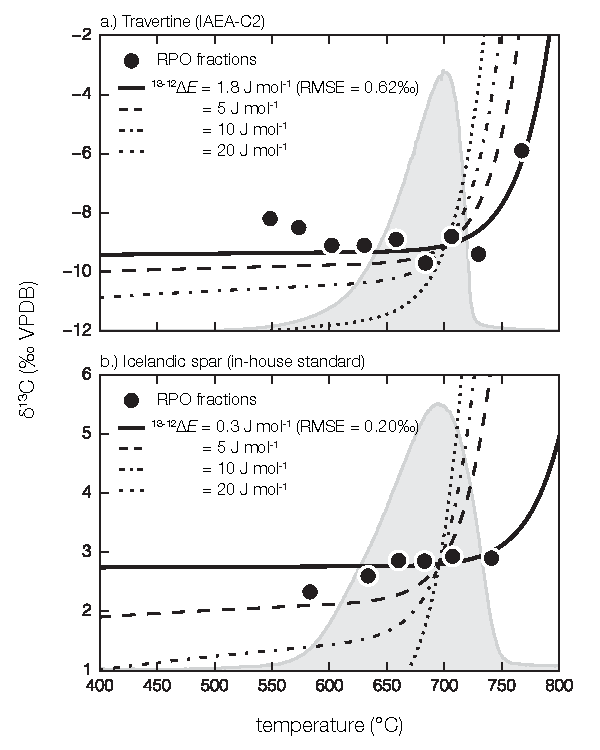
\includegraphics[]{Thesis_Figures/Ch2Fig5}}
	\caption[SRM kinetic isotope fractionation results]{RPO fraction $\delta^{13}$C values for two carbonate SRMs [$(A)$ travertine and $(B)$ Icelandic spar] plotted with the predicted $\delta^{13}$C value at each temperature using best-fit $\Delta E$ values from Equation \ref{Ch2Eq:13} (solid black line). For reference, predicted $\delta^{13}$C values for various $\Delta E$ values are plotted as dashed and dotted lines, while shaded gray regions represent normalized thermograms (unitless). Each RPO fraction is plotted at its CO\textsubscript{2}-mass-weighted mean temperature.}
	\label{Ch2Fig:5} 
\end{figure}

Furthermore, if kinetic fractionation were driving observed \ce{^{13}C} variability, \ce{\delta^{13}C} values of eluted \ce{CO2} from all samples should increase monotonically with temperature along a trend that depends only on $\Delta E$, which is clearly not observed. Rather, the \ce{\delta^{13}C} spread (\textit{i.e.} max -- min) across RPO fractions is highly variable between samples, reaching values as high as $28.8$\textperthousand\ in carbonate-containing lacustrine sediments and as low as $0.3$\textperthousand\ in decarbonated soils. For three carbonate-containing sediments analyzed here, we additionally measured the \ce{\delta^{13}C} value of total inorganic carbon following standard methods \citep{McNichol:1994ty} to compare with blank and mass-balance corrected RPO results. For all samples, high-temperature RPO \ce{\delta^{13}C} values agree with those of total inorganic carbon to within $1$\textperthousand, further indicating that RPO \ce{\delta^{13}C} values accurately reflect source carbon composition. 

Lastly, decreasing \ce{\delta^{13}C} values have been observed with increasing temperature in select samples such as decarbonated Ganges River total suspended sediments and Hawaiian soils (Figure \ref{Ch2Fig:6}), opposite of trends that would depict kinetic fractionation. Rather, this agrees with the interpretation that labile C\textsubscript{3} OC in these environments is replaced by \ce{^{13}C}-enriched, C\textsubscript{4}-derived material \citep{Chadwick:2007hc,Galy:2008jw}, and is further evidence that measured \ce{\delta^{13}C} trends reflect differences in carbon source isotope composition. Combined, the RPO \ce{\delta^{13}C} trends from environmental samples analyzed here agree with SRM-based fractionation predictions indicating that kinetic fractionation is small (\textit{i.e.} less than $1 - 2$\textperthousand) in the RPO instrument at NOSAMS.

% Figure 6
\begin{figure}[t]
	\makebox[\textwidth][c]{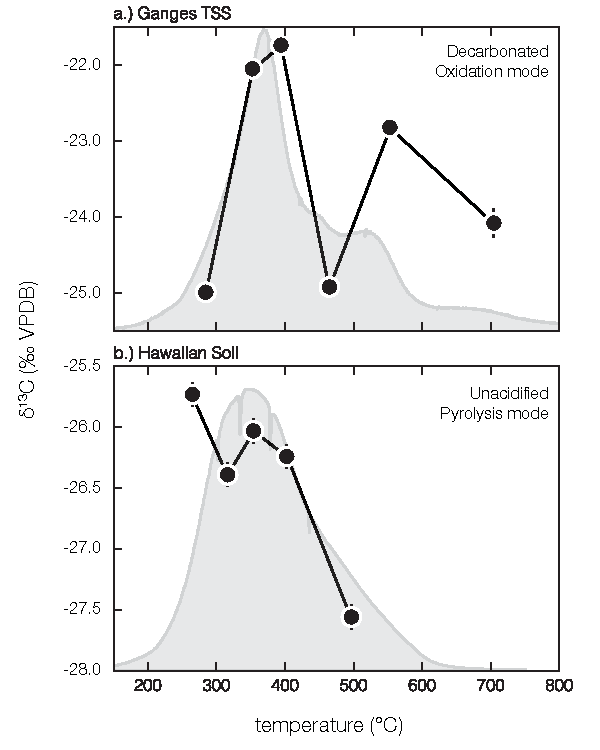
\includegraphics[]{Thesis_Figures/Ch2Fig6}}
	\caption[Samples exemplifying decreasing \ce{\delta^{13}C} with temperature]{RPO fraction \ce{\delta^{13}C} values for two environmental samples: $(A)$ decarbonated Ganges River TSS and $(B)$ Hawaiian soil. \ce{\delta^{13}C} values do not show a monotonic increase with temperature, precluding the possibility that \ce{^{13}C} variability in these samples reflects kinetic fractionation. For reference, shaded gray regions represent normalized thermograms (unitless). Each RPO fraction is plotted at its \ce{CO2}-mass-weighted mean temperature.}
	\label{Ch2Fig:6} 
\end{figure}

\section{Conclusion}

We describe the blank carbon composition, isotope mass balance, and kinetic isotope fractionation within the NOSAMS RPO instrument. Blank carbon mass is significantly smaller than that reported on a similar system \citep{Fernandez:2014gx} and can be described as a constant flux of $4.5 \pm 0.7$ ngC \textdegree C\textsuperscript{-1} (for a $5$\textdegree C min\textsuperscript{-1} ramp rate) with an Fm value of $0.555 \pm 0.042$ and a \ce{\delta^{13}C} value of $-29.0 \pm 0.1$\textperthousand. We find no evidence for significant time-independent blank contribution, likely due to recent valve and plumbing upgrades within the instrument \citep{Plante:2013tu}.

Isotope mass balance on a suite of environmental samples indicates that independently measured bulk Fm is accurately reconstructed using the RPO fraction mass-weighted mean. In contrast, RPO-predicted weighted-average \ce{\delta^{13}C} values are slightly depleted relative to measured bulk \ce{\delta^{13}C} values, especially for decarbonated samples containing exclusively OC. We eliminate the possibility that this depletion is due to low carbon yield or fractionation within the toggling traps. Rather, we hypothesize that this is caused by incomplete oxidation of reduced gases to \ce{CO2} within the oxidation oven and suggest that \ce{\delta^{13}C} of each RPO fraction for a given sample can be mass-balance corrected using the difference between measured bulk and mass-weighted mean values of that sample.

High-resolution \ce{\delta^{13}C} measurements on two carbonate SRMs suggest that kinetic isotope fractionation cannot exceed $1.8$\textperthousand\ in the RPO instrument. This agrees with intra-sample \ce{^{13}C} trends of the environmental samples analyzed for this study, which display a large range in \ce{\delta^{13}C} spread between fractions and are consistent with independently measured carbon source composition. Additionally, selected samples display \ce{^{13}C} trends with temperature opposite of that predicted by kinetic fractionation. These results are strong evidence that RPO kinetic fractionation is small and that blank and mass-balance corrected \ce{\delta^{13}C} values of each \ce{CO2} fraction reflect carbon source isotope composition to within $1 - 2$\textperthousand.

%\section{Acknowledgements}

%We thank Carl Johnson and the NOSAMS sample-prep lab staff for laboratory assistance. Instrumental improvements to the RPO system were largely the work of Steven Beaupr�. V.V.G. was partly supported by the US National Science Foundation (grants OCE-0851015 and OCE-0928582), the WHOI Coastal Ocean Institute (grant 27040213) and an Independent Study Award (grant 27005306) from WHOI; J.D.H. was partly supported by the NSF Graduate Research Fellowship Program under grant number 2012126152; G.S. and P.K.Z. were supported by the WHOI Postdoctoral Scholar Program with funding provided by NOSAMS.
